\subsection{Heat Maps}
	This section will cover all the aspects of the heat maps use case (Figure \ref{HeatMapUseCase}). This use case is chosen as it is a vital part of the entire system. The data that is recorded will be used to create the heat maps that can then later be used to analyse the data and be used for future uses.
	\newline
	\begin{figure}[!ht]
		\centering
		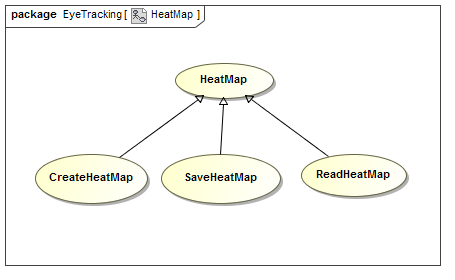
\includegraphics[scale=0.5]{Diagrams/Use_Case_Diagram__HeatMap.png}
		\caption{Heat Map Use Case}
		\label{HeatMapUseCase}
	\end{figure}
	

	The following sub use cases are included in this use case:
	\subsubsection{CreateHeatMap}
The create heat map use case deals with the creation of the heat map from the recorded data. The heat map shows where on the media item has been viewed the most by the user(s).
	\begin{itemize}
		\item Pre-condition: Data must be already recorded.
		\item Post-condition: Heat map of the data is created.
		\item Request Data Structure: HeatMap.CreateHeatMap(Data[]).
		\item Return data Structure: Heatmap is created
	\end{itemize}
	\begin{figure}[!ht]
		\centering
		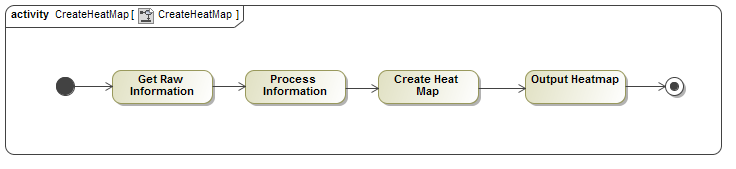
\includegraphics[scale=0.5]{Diagrams/Activity_Diagram__CreateHeatMap__CreateHeatMap.png}
		\caption{Create Heat Map Activity}
	\end{figure}
	
	\subsubsection{ReadHeatMap}
	This use case deals with the viewing of Heat maps from their recorded data. Once the heat map is created the users will be able to see the heat map and view the data.
	\begin{itemize}
		\item Pre-condition: Heat map must have been created.
		\item Post-condition: Heat map of the data is viewable and can be further analysed.
		\item Request Data Structure: HeatMap.ReadHeatMap(heatmapID).
		\item Return Data Structure: Heat map is viewable.
	\end{itemize}
	
	\begin{figure}[!ht]
		\centering
		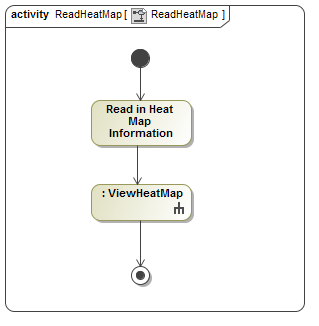
\includegraphics[scale=0.5]{Diagrams/Activity_Diagram__ReadHeatMap__ReadHeatMap.png}
		\caption{Read Heat Map Activity}
	\end{figure}
	
	\subsubsection{SaveHeatMap}
	This use case deals with the saving of heat maps that are created from their respective recorded data. The heat map will be saved on the users computer to be viewed at a later date. This will save only the heat map which can later be saved onto a model at a later date.
	\begin{itemize}
		\item Pre-condition: Heat map must have been created.
		\item Post-condition:Heat map of the data is saved.
		\item Request Data Structure:HeatMap.SaveHeatMap(Data[]).
		\item Return Data Structure:Heatmap is saved.
	\end{itemize}
	
	\begin{figure}[!ht]
		\centering
		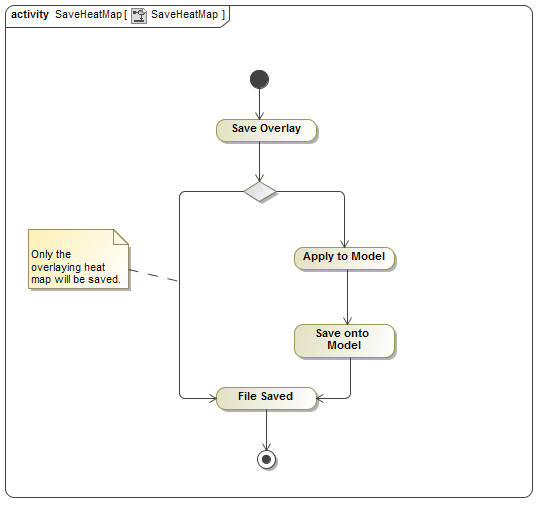
\includegraphics[scale=0.5]{Diagrams/Activity_Diagram__SaveHeatMap__SaveHeatMap.png}
		\caption{Save Heat Map Activity}
	\end{figure}
	
\subsection{Save Heat Maps}
	The saving of the heat maps provides important functionality to the system as it will allow the users to save the data which can later be used to either continue research or to compare data.The heat map will serve as an overlay for the media type and be placed over the media model. The saving of heat maps can be divided into three subsections, namely SaveOn2DModel, SaveOnVideo and SaveOn3DModel.
	\newline
	
	\begin{figure}[!ht]
		\centering
		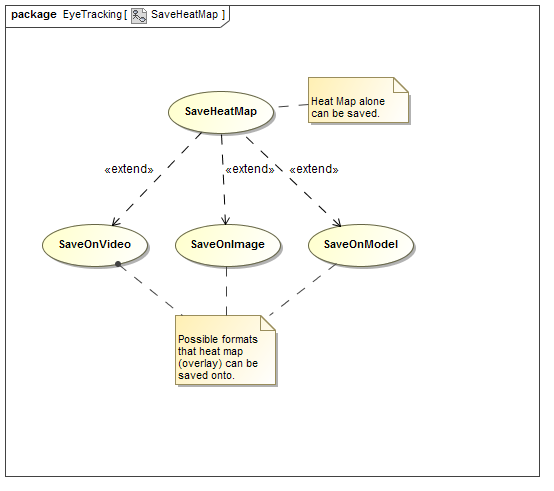
\includegraphics[scale=0.5]{Diagrams/Use_Case_Diagram__SaveHeatMap.png}\newline
		\caption{Save Heat Map Use Case}
	\end{figure}		
		
	
	\subsubsection{SaveOn2DModel}
The heat map that is created for a 2D model media type will be saved and applied to the 2D model to see the heat map over the model to indicate what has been viewed the most by the users.
	\begin{itemize}
		\item Pre-condition: Heat map must have been created and the 2D model of the heat map must be available.
		\item Post-condition: Heat map of the data is viewable on the 2D model as an overlay.
		\item Request Data Structure: HeatMap.SaveOn2DModel(heatmapID,2DModelID).
		\item Return Data Structure: Heat map of the data is placed over the 2DModel.
	\end{itemize}
	\begin{figure}[!ht]
		\centering	
		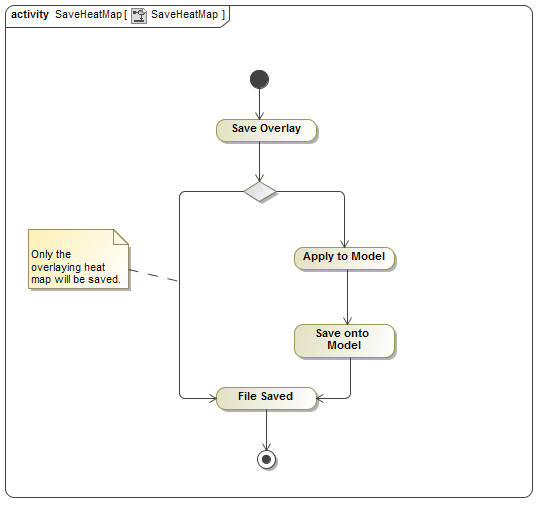
\includegraphics[scale=0.5]{Diagrams/Activity_Diagram__SaveHeatMap__SaveHeatMap.png}	
		\caption{Save on 2D Model Activity}
	\end{figure}

	\subsubsection{SaveOnVideo}
	The heat map that is created for a video media type will be saved and then applied to the video to see the heat map over the video to indicate what has been viewed the most by the users. The heat map will follow the video as the video plays and be changed as time passes.
	\begin{itemize}
		\item Pre-condition: Heat map must have been created and the video must be available.
		\item Post-condition: Heat map of the data is viewable on the video as an overlay and tracks the video position to be changed as the video plays.
		\item Request Data Structure: HeatMap.SaveOnImage(heatmapID,ImageID).
		\item Return Data Structure: Heat map of the data is placed over the video.
	\end{itemize}
	\begin{figure}[!ht]
		\centering	
		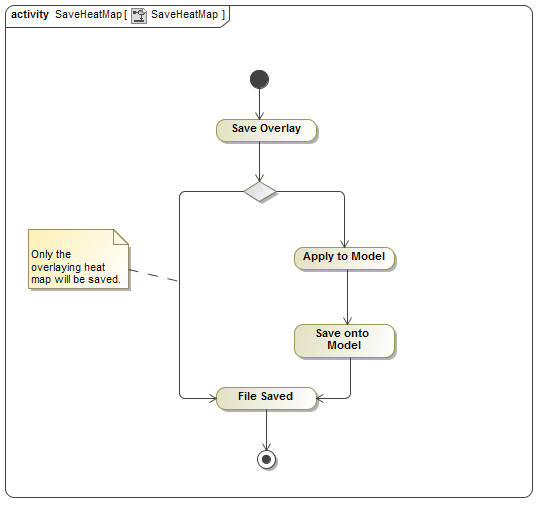
\includegraphics[scale=0.5]{Diagrams/Activity_Diagram__SaveHeatMap__SaveHeatMap.png}	
		\caption{Save on Video Model Activity}
	\end{figure}

	\subsubsection{SaveOn3DModel}
	The heat map that is created for a 3D model media type will be saved and then applied to the 3D model to see the heat map over the 3D model to indicate what has been viewed the most by the users. The 3D model with heat map overlay can be saved as either a 2D or 3D model.
	\begin{itemize}
		\item Pre-condition: Heat map must have been created and the 3D model of the heat map must be available.
		\item Post-condition: Heat map of the data is viewable on the 3D model as an overlay.
		\item Request Data Structure: HeatMap.SaveOn3DModel(heatmapID,3DModelID).
		\item Return Data Structure: Heat map of the data is placed over the 3D model.
	\end{itemize}
	\begin{figure}[!ht]
		\centering	
		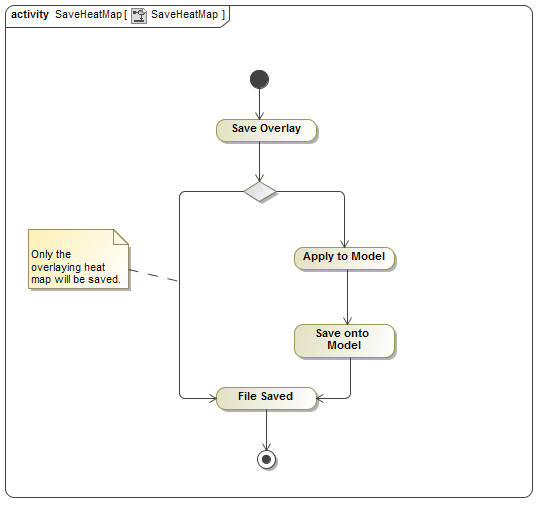
\includegraphics[scale=0.5]{Diagrams/Activity_Diagram__SaveHeatMap__SaveHeatMap.png}	
		\caption{Save on 3D Model Activity}
	\end{figure}
		
\subsection{Models}
This section details all the different types of media or models that heat maps can be created for and saved onto. There are three types of models, namely Video, 2D and 3D. The heat maps are created based on the models and their types.
\newline
\begin{figure}[!ht]
	\centering	
	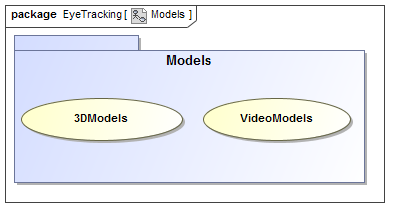
\includegraphics[scale=0.5]{Diagrams/Use_Case_Diagram__Models.png}
	\caption{Models Use Case}
\end{figure}
	
	\subsubsection{3D Models}
	3D Models will be opened and rendered by the system, and will then be made viewable to the user. The heat map can then be saved onto the model as well as opened as the stand alone heat map.
	\newline
	\begin{figure}[!ht]
		\centering
		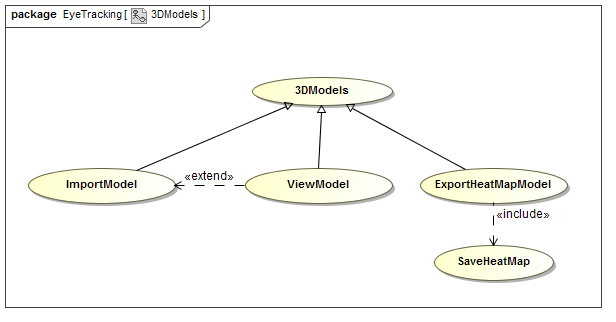
\includegraphics[scale=0.5]{Diagrams/Use_Case_Diagram__3DModels.png}
		\caption{3D Models Use Case}
	\end{figure}
	
	\begin{enumerate}
		\item{ImportModel}
		\newline
		This will allow for a 3D model media type to be imported into the system for further processing. The imported model can be used for recording data onto and creating a relevant heat map based on it which can then be applied to it at a later stage.
		\begin{itemize}
			\item Pre-condition: 3D model must exist.
			\item Post-condition: Recording can be done on the model.
			\item Request Data Structure: HeatMap.3DModeImport(3DModelID).
			\item Return Data Structure: Rendered data model is imported.
		\end{itemize}
		
		\begin{figure}[!ht]
			\centering
			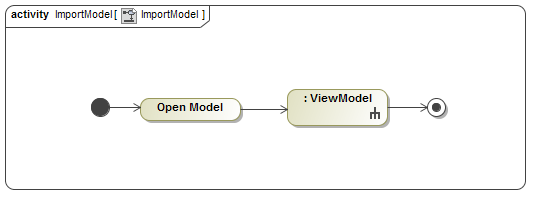
\includegraphics[scale=0.5]{Diagrams/Activity_Diagram__ImportModel__ImportModel.png}
			\caption{Import 3D Model Activity}
		\end{figure}
	
		\item{ViewModel}
		Once the model is imported the model will be rendered for viewing and further processing decided by the user.
		\begin{itemize}
			\item Pre-condition: 3D model must have been imported .
			\item Post-condition: 3D model is viewable and can be recorded on.
			\item Request Data Structure: HeatMap.View3DModel(3DModelID).
			\item Return Data Structure: Viewable 3D model
		\end{itemize}
		\begin{figure}[!ht]
			\centering
			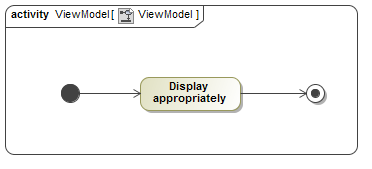
\includegraphics[scale=0.5]{Diagrams/Activity_Diagram__ViewModel__ViewModel.png}
		\caption{View 3D Model Activity}
		\end{figure}
		
		\item{ExportHeatMapModel}
		The exported model will have the heat map applied to it which can then be exported as a new 3D model so that it can be viewed or used at a later date by the user. 
		\begin{itemize}
			\item Pre-condition: Heat Map must be created and Model Imported.
			\item Post-condition: Exported Model With heatmap on it to be viewed.
			\item Request Data Structure: HeatMap.ExportHeatMap3DModel(heatmapID,3DModelID).
			\item Return Data Structure: Model with heat map.
		\end{itemize}
		
		\begin{figure}[!ht]
			\centering
			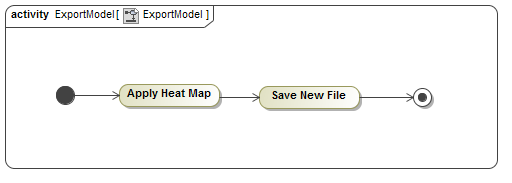
\includegraphics[scale=0.5]{Diagrams/Activity_Diagram__ExportModel__ExportModel.png}
			\caption{Export 3D Model Activity}
		\end{figure}
	\end{enumerate}

	\subsubsection{2D Models}
	2D models will typically refer to images but can also refer to any media that is does not show a third dimension of movement but for the scope of this project will only refer to images. The heat map can then be created and applied to the image.
	\newline
	\begin{figure}[!ht]
		\centering
		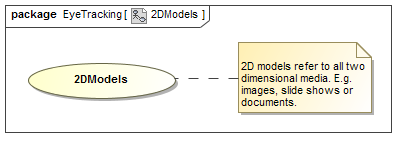
\includegraphics[scale=0.5]{Diagrams/Use_Case_Diagram__2DModels.png}
		\caption{2D Models Use Case}
	\end{figure}
	\begin{enumerate}
		\item{ImportModel}
		\newline
		The 2D models can be imported into the system which can then be process further by the user. The imported model can then have recordings done and heat maps created for it. 
		\begin{itemize}
			\item Pre-condition: 2D model must exist, a image preferable.
			\item Post-condition: Recording can be done on the model.
			\item Request Data Structure: HeatMap.2DModeImport(2DModelID).
			\item Return Data Structure: Rendered image is imported.
		\end{itemize}
		
		\begin{figure}[!ht]
			\centering
			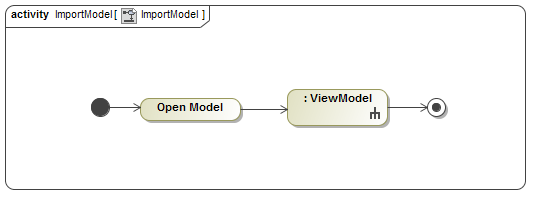
\includegraphics[scale=0.5]{Diagrams/Activity_Diagram__ImportModel__ImportModel.png}
			\caption{Import 2D Model Activity}
		\end{figure}
	
		\item{ViewModel}
		Once the model is imported the users can view the model and eye tracking can then be applied on the model. The model can the be processed further as the user sees fit.
		\begin{itemize}
			\item Pre-condition: 2D model (image) must have been imported.
			\item Post-condition: Image is viewable and can be recorded on.
			\item Request Data Structure: HeatMap.View2DModel(2DModelID)
			\item Return Data Structure: Viewable image.
		\end{itemize}
		
		\begin{figure}[!ht]
			\centering
			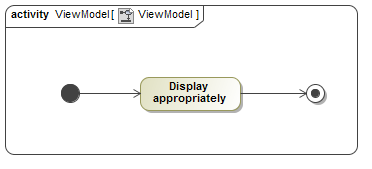
\includegraphics[scale=0.5]{Diagrams/Activity_Diagram__ViewModel__ViewModel.png}
			\caption{View 2D Model Activity}
		\end{figure}
	
		\item{ExportHeatMapModel}
		The exported model will have the heat map applied to it which can then be exported as a new 2D model so that it can be viewed or used at a later date by the user.  
		\begin{itemize}
			\item Pre-condition: Heat Map must be created and Model Imported.
			\item Post-condition: Exported Model With heatmap on it to be viewed.
			\item Request Data Structure: HeatMap.Export2Dmodel(2DModelID).
			\item Return Data Structure: Model with heat map.
		\end{itemize}
		
		\begin{figure}[!ht]
			\centering
			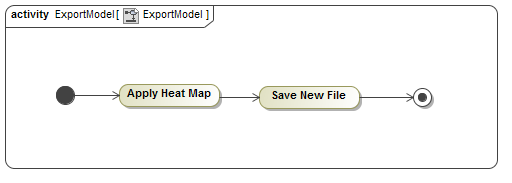
\includegraphics[scale=0.5]{Diagrams/Activity_Diagram__ExportModel__ExportModel.png}
			\caption{Export 2D Model Activity}
		\end{figure}
	
	\end{enumerate}
		
		
	\subsubsection{Video Models}
	A video can be easily imported into the system. Eye tracking can then be done to the video model and the recorded data can be stored. The data can then be used to create a heat map that can then be applied to the video second by second.
	\newline
	
	\begin{figure}[!ht]
		\centering
		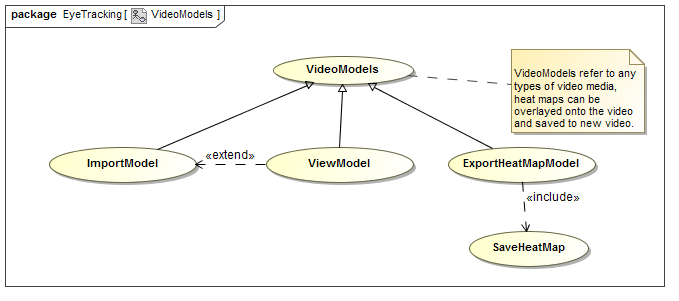
\includegraphics[scale=0.5]{Diagrams/Use_Case_Diagram__VideoModels.png}
		\caption{Video Models Use Case}
	\end{figure}
	
		\begin{enumerate}
			\item{ImportModel}
			\newline
			The video models can be imported into the system which can then be process further by the user. The imported model can then have recordings done and heat maps created for it. Heat maps that will be recorded will show a second by second representation of the heat map data.
			\begin{itemize}
				\item Pre-condition: video must exist.
				\item Post-condition: Recording can be done on the video.
				\item Request Data Structure: HeatMap.VideoImport(videoID).
				\item Return Data Structure: Rendered video is imported.
			\end{itemize}
			
			\begin{figure}[!ht]
				\centering
				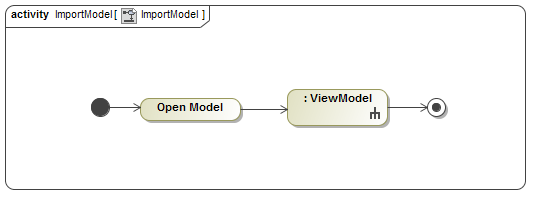
\includegraphics[scale=0.5]{Diagrams/Activity_Diagram__ImportModel__ImportModel.png}
				\caption{Import Video Model Activity}
			\end{figure}
			
			\item{ViewModel}
Once the model is imported the users can view the model and eye tracking can then be applied on the model. The model can the be processed further as the user sees fit.
			\begin{figure}
				\centering
				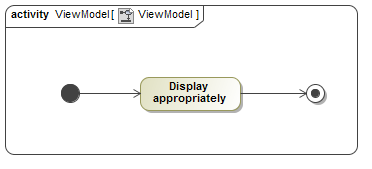
\includegraphics[scale=0.5]{Diagrams/Activity_Diagram__ViewModel__ViewModel.png}
				\caption{View Video Model Activity}
			\end{figure}
			
			
			
			\item{ExportHeatMapModel}
			The exported model will have the heat map applied to it which can then be exported as a new video model so that it can be viewed or used at a later date by the user. The exported video model will have the heat map recorded onto the original video and saved in the appropriate format.
			\begin{itemize}
				\item Pre-condition: Heat map must be created and video imported.
				\item Post-condition: Exported video With heat map on it to be viewed.
				\item Request Data Structure: HeatMap.SaveOnvideo(videolID).
				\item Return Data Structure: Video with heat map.
			\end{itemize}
		\begin{figure}[!ht]
			\centering
			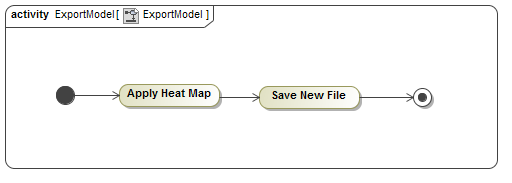
\includegraphics[scale=0.5]{Diagrams/Activity_Diagram__ExportModel__ExportModel.png}
			\caption{Export 3D Model Activity}
		\end{figure}
	
		\end{enumerate}
		
%=========================================================%		
\subsection{Raw Information}
When recording happens on the system the raw information is saved. The raw information is important as it forms the basis for creating heat maps and statistics for specific models. The raw information is can be saved on the system and processed further by the user. The raw information can then be read as the raw data or put into a statistical formats.
\newline

\begin{figure}[!ht]
	\centering
	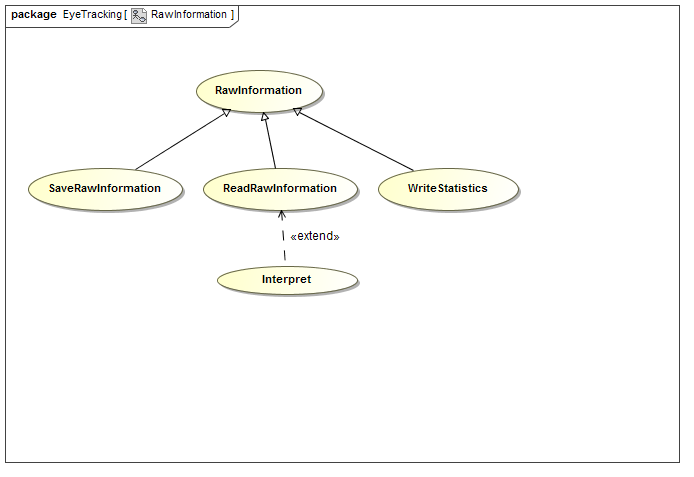
\includegraphics[scale=0.5]{Diagrams/Use_Case_Diagram__RawInformation.png}
	\caption{Raw Information Use Case}
\end{figure}
	
	\subsubsection{SaveRawInformation}
When recording is done on the media the raw information will need to be saved so that it can be used at a later stage. This raw information can then be reopened later for the relevant model and used by user for further processing and interpretation.
\begin{itemize}
\item Pre-condition: Recording on a media type must have happened.
\item Post-condition: Data is saved and can be used later.
\item Request Data Structure: HeatMap.SaveRawInformation(data[]).
\item Return Data Structure: Raw array of data points saved.
\end{itemize}

\begin{figure}[!ht]
	\centering
	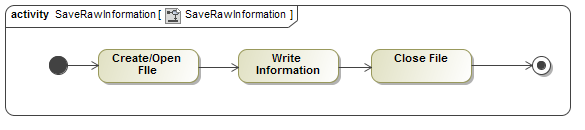
\includegraphics[scale=0.5]{Diagrams/Activity_Diagram__SaveRawInformation__SaveRawInformation.png}
	\caption{Save Raw Information Activity}
\end{figure}

	\subsubsection{ReadRawInformation}
Data can be read from a previously saved file. This will allow the user to import the raw information for the relevant model which can then be used for comparison or further processing.
\begin{itemize}
\item Pre-condition: Recorded data must be saved in a file.
\item Post-condition: Data is displayed.
\item Request Data Structure: HeatMap.ReadRawInformation(file).
\item Return Data Structure: data array with all data points.
\end{itemize}

\begin{figure}[!ht]
	\centering
	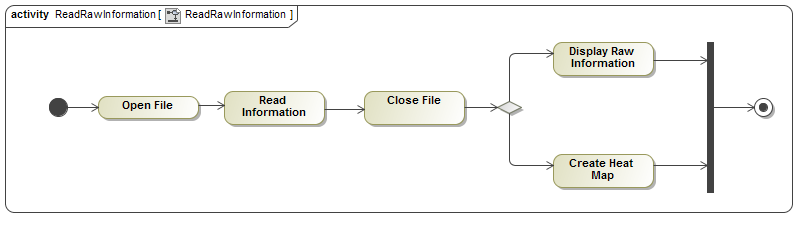
\includegraphics[scale=0.5]{Diagrams/Activity_Diagram__ReadRawInformation__ReadRawInformation.png}
	\caption{Read Raw Information Activity}
\end{figure}
	
	\subsubsection{CreateStatistics}
The writing of statistics is part of the Statistics use-case and all information can be found there regarding the sub use case

	
	
\subsection{Statistics}
Statistics on all the data will be collected and will then be used to make a statistical page based off the model that can be analysed and then it can be easily compared at any time.
\newline
\begin{figure}[!ht]
	\centering
	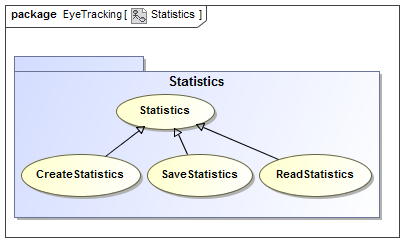
\includegraphics[scale=0.5]{Diagrams/Use_Case_Diagram__Statistics.png}
	\caption{Statistics Use Case}
	\end{figure}
	
		\subsubsection{CreateStatistics}
Using the recorded data we can create statistical data which can then be used for analysis. This data can then be viewed or used to compared data.
\begin{itemize}
\item Pre-condition: Recorded data must exist.
\item Post-condition: Data is turned into statistical data.
\item Request Data Structure: Stats.CreateStats(data[]).
\item Return Data Structure: Statistics in arrays.
\end{itemize}

\begin{figure}[!ht]
	\centering
	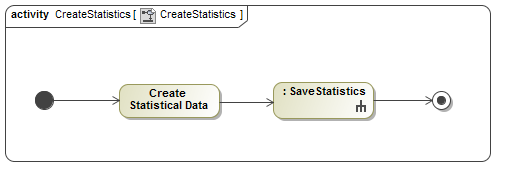
\includegraphics[scale=0.5]{Diagrams/Activity_Diagram__CreateStatistics__CreateStatistics.png}
	\caption{Create Statistics Activity}
	\end{figure}
	
		\subsubsection{SaveStatistics}
The statistical data can be saved into a file so that they can be printed out and be used as a hard copy. This will take all data and save it to a pdf or csv file.
\begin{itemize}
\item Pre-condition: Statistical data must exist.
\item Post-condition: Data is put into a report.
\item Request Data Structure: Stats.SaveStats(statsdata[]).
\item Return Data Structure: Save report in pdf or csv format.
\end{itemize}

\begin{figure}[!ht]
	\centering
	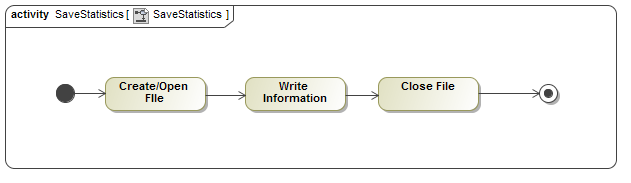
\includegraphics[scale=0.5]{Diagrams/Activity_Diagram__SaveStatistics__SaveStatistics.png}
	\caption{Save Statistics Activity}
	\end{figure}
	
\subsection{Record Eyes}
The recording of the eyes will be done using the Eye Tribe camera or any other eye tracking camera. The data recorded in this process will allow heat maps and statistics to be generated. The heat maps can then be turned into overlays for the appropriate media types. The record eye use case (Figure \ref{RecordEye}) makes use of sub use cases from other use cases that are listed below, such as SaveRawInformation. The recording of the information is important as this is used throughout the project and its functionality.
\newline

\begin{figure}[!ht]
	\centering 
	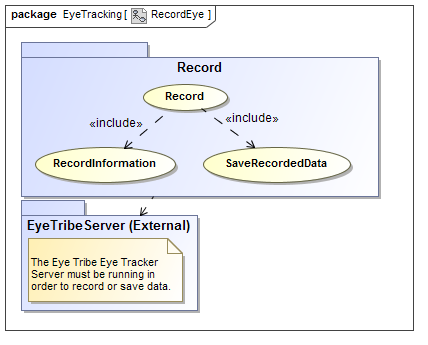
\includegraphics[scale=0.5]{Diagrams/Use_Case_Diagram__RecordEye.png}
	\caption{Record Eye Use Case}
	\label{RecordEye}
	\end{figure}
	
\subsubsection{RecordInformation}
The recorded information will be sent to the OGAMA module to be processed and interpreted, which will then return the relevant information which can then be used to carry out functions in the system.
The
\begin{itemize}
\item Pre-condition: User needs to look at the media.
\item Post-condition: Data is recorded about the eye movements.
\item Request Data Structure: Recorder.Record(type).
\item Return Data Structure: Raw data in x, y and z co ordinates.
\end{itemize}

\begin{figure}[!ht]
	\centering
	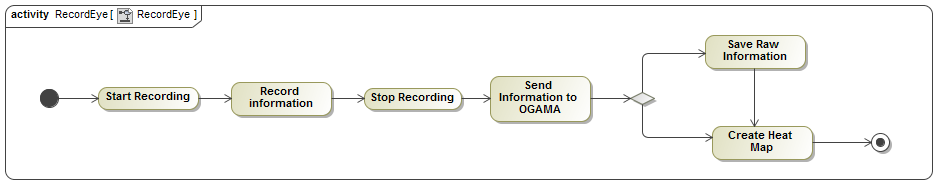
\includegraphics[scale=0.5]{Diagrams/Activity_Diagram__RecordEye__RecordEye.png}
	\caption{Record Eye Activity}
	\end{figure}

